\documentclass[twoside]{article}
\usepackage[utf8]{inputenc}
\usepackage[ngerman]{babel}
\usepackage{libertine}
\usepackage[dvipsnames]{xcolor}
\usepackage[a4paper]{geometry}
\usepackage{pdfpages}
\usepackage{parskip}
\usepackage{amsmath, amsthm, amssymb, commath, mathtools}
\usepackage{cancel}
\usepackage{physics}
\usepackage[version=4]{mhchem}
\usepackage{nicefrac}
\usepackage{booktabs}
\usepackage{tabularx}
\usepackage{tabu}
\usepackage{enumitem}
\usepackage{graphicx}
\graphicspath{{./plots/}{./images/}}
\usepackage{wrapfig}
\definecolor{capblue}{HTML}{00709B}
\usepackage[margin=1cm,font={small},labelfont={color=capblue}]{caption}
\usepackage{subcaption}
\usepackage{float}
\usepackage{minted}
\usepackage{appendix}
\usepackage{icomma}
\usepackage{multirow}
\usepackage{multicol}
\usepackage{footmisc}
\usepackage[separate-uncertainty=true]{siunitx}
\sisetup{locale = DE}
\usepackage{tcolorbox}

\usepackage{ccicons}

\usepackage{csquotes}
\MakeOuterQuote{"}
\renewcommand{\ttdefault}{cmtt}

\usepackage{hyperref}
\usepackage{bookmark}
% https://tex.stackexchange.com/a/33701
\makeatletter
    \newcommand{\nonum}[0]{%
        \let\@oldseccntformat\@seccntformat %
        \renewcommand\@seccntformat[1]{}%
        }
    \newcommand{\resnum}[0]{\let\@seccntformat\@oldseccntformat}
\makeatother

\usepackage{chngcntr}
\counterwithin{figure}{section}
\counterwithin{table}{section}

\usepackage[style=iso-authoryear,sortcites=true,sorting=nyt,backend=biber,language=ngerman,natbib=true,sortlocale=de_DE]{biblatex}
\addbibresource{references.bib}
\newcommand{\mkbibbracketscol}[1]{\textcolor{gray}{\mkbibbrackets{#1}}}
\DeclareCiteCommand{\cite}[\mkbibbracketscol]
  {\usebibmacro{prenote}}
  {\usebibmacro{citeindex}%
   \usebibmacro{cite}}
  {\multicitedelim}
  {\usebibmacro{postnote}}

\DeclareCiteCommand{\parencite}[\mkbibbracketscol]
  {\usebibmacro{prenote}}
  {\usebibmacro{citeindex}%
   \usebibmacro{cite}}
  {\multicitedelim}
  {\usebibmacro{postnote}}


\DeclareCiteCommand{\cbx@textcite}[\textcolor{gray}]
  {\usebibmacro{textcite:init}}
  {\usebibmacro{citeindex}%
   \usebibmacro{textcite}}
  {}
  {\usebibmacro{textcite:postnote}}

\DefineBibliographyStrings{ngerman}{%
    bibliography    = {Literaturverzeichnis},
    andothers       = {u.\,a.\adddot}
}

\let\realcitep\citep
\renewcommand*{\citep}[1]{{\footnotesize\realcitep{#1}}}

\newcommand{\versuch}[0]{QAL}
\newcommand{\versuchLang}[0]{Quantum Analogs}

\hypersetup{
	pdftitle={P3B -- \versuch{} Auswertung},
	pdfauthor={Yudong Sun},
	bookmarksnumbered=true,
	bookmarksopen=true,
	bookmarksopenlevel=2,
	pdfstartview=Fit,
	pdfpagemode=UseOutlines,
	colorlinks=true,
	linkcolor=black,
	filecolor=magenta,      
	urlcolor=blue,
    citecolor=gray
}
\urlstyle{same}

\title{\versuch{} -- \versuchLang \\ Auswertung}
\author{Yudong Sun\\Gruppe L8}

\usepackage{fancyhdr}
\pagestyle{fancy}
\fancyhf{}
\fancyhead[RO]{Yudong Sun}
\fancyhead[LO]{Auswertung -- \versuch}
\fancyhead[LE]{Yudong Sun}
\fancyhead[RE]{Auswertung -- \versuch}
\cfoot{\thepage}

% Custom Defs
\newcommand*{\ra}[1]{\renewcommand{\arraystretch}{#1}}
\newcommand*{\maxi}[1]{\text{max}\left(#1\right)}
\newcommand*{\mini}[1]{\text{min}\left(#1\right)}
\newcommand*{\todo}[1]{\textcolor{red}{TODO: #1}}
\newcommand*{\iu}[1]{\textit{\underline{#1}}}
\newcommand*{\gnuplot}[0]{\texttt{gnuplot}}
\newcommand*{\captionbr}[0]{\\\rule{\textwidth}{0pt}\\\vspace{-\baselineskip}}
\newcommand*{\sigfig}[1]{\hspace{0.5cm}\text{(#1 sig. Zif.)}}
\newcommand*{\pbrace}[1]{\left(#1\right)}
\newcommand*{\sbrace}[1]{\left[#1\right]}
\newcommand*{\bDelta}[1]{\pbrace{\Delta #1}}
\newcommand*{\overbar}[1]{\overline{\raisebox{0pt}[1.2\height]{$#1$}}} % https://tex.stackexchange.com/a/87615
\newenvironment{beispiel}
    {\begin{tcolorbox}[title=Beispielrechnung]}
    {\end{tcolorbox}}

\newcommand*{\realzahl}[0]{\mathbb{R}}
\newcommand*{\natzahl}[0]{\mathbb{N}}
\newcommand*{\ratzahl}[0]{\mathbb{Q}}
\newcommand*{\intzahl}[0]{\mathbb{Z}}
\newcommand*{\boolzahl}[0]{\mathbb{B}}

\newcommand*{\question}[1]{\textit{\textcolor{Magenta}{#1}}}

% \addto\captionsngerman{
%     \let\oldfigname\figurename
%     \renewcommand{\figurename}{[\oldfigname}
%     \let\oldthefig\thefigure
%     \renewcommand{\thefigure}{\oldthefig]}
% } % https://tex.stackexchange.com/a/17490
% https://tex.stackexchange.com/a/101624 new line in caption

% Gaußsche Fehler Erzeuger
\makeatletter
    \newcommand{\gausserror}[2]{% \gausserror{G}{faktoren}
        \sqrt{%
            \@tempswafalse
            \@for\factor:=#2
            \do{
                \if@tempswa+%
                \else%
                    \@tempswatrue%
                \fi%
                \left(\pdv{#1}{\factor}\Delta\factor\right)^2%
            }%
        }
    }
\makeatother
% https://tex.stackexchange.com/a/59912
% https://riptutorial.com/latex/example/28657/loops---repeating-things

% Add quad
\makeatletter
    \newcommand{\addquad}[1]{% \gausserror{G}{faktoren}
        \sqrt{%
            \@tempswafalse
            \@for\factor:=#1
            \do{
                \if@tempswa+%
                \else%
                    \@tempswatrue%
                \fi%
                \left(\Delta\factor\right)^2%
            }%
        }
    }
\makeatother

% rej quad
\makeatletter
    \newcommand{\relquad}[1]{% \gausserror{G}{faktoren}
        \sqrt{%
            \@tempswafalse
            \@for\factor:=#1
            \do{
                \if@tempswa+%
                \else%
                    \@tempswatrue%
                \fi%
                \left(\frac{\Delta\factor}{\factor}\right)^2%
            }%
        }
    }
\makeatother

\newcommand*{\ub}[1]{\underbracket[0.1ex]{#1}}
\newcommand*{\ob}[1]{\overbracket[0.1ex]{#1}}
\newcommand*{\brc}[2]{\mathrlap{\ub{\phantom{#1}}_{#2}}#1}
\newcommand*{\brd}[2]{\mathrlap{\ob{\phantom{#1}}^{#2}}#1}

% / Custom Defs

\begin{document}

\maketitle

% Einstellungen
\nonum
\numberwithin{equation}{section}
% / Einstellungen

\section{Teilversuch 1: Bragg Reflexion von Röntgenstrahlung des Molybdän an einem \ce{NaCl}-Einkristall}
	\begin{figure}[!ht]
		\centering
		\begin{subfigure}{0.48\textwidth}
			\centering
			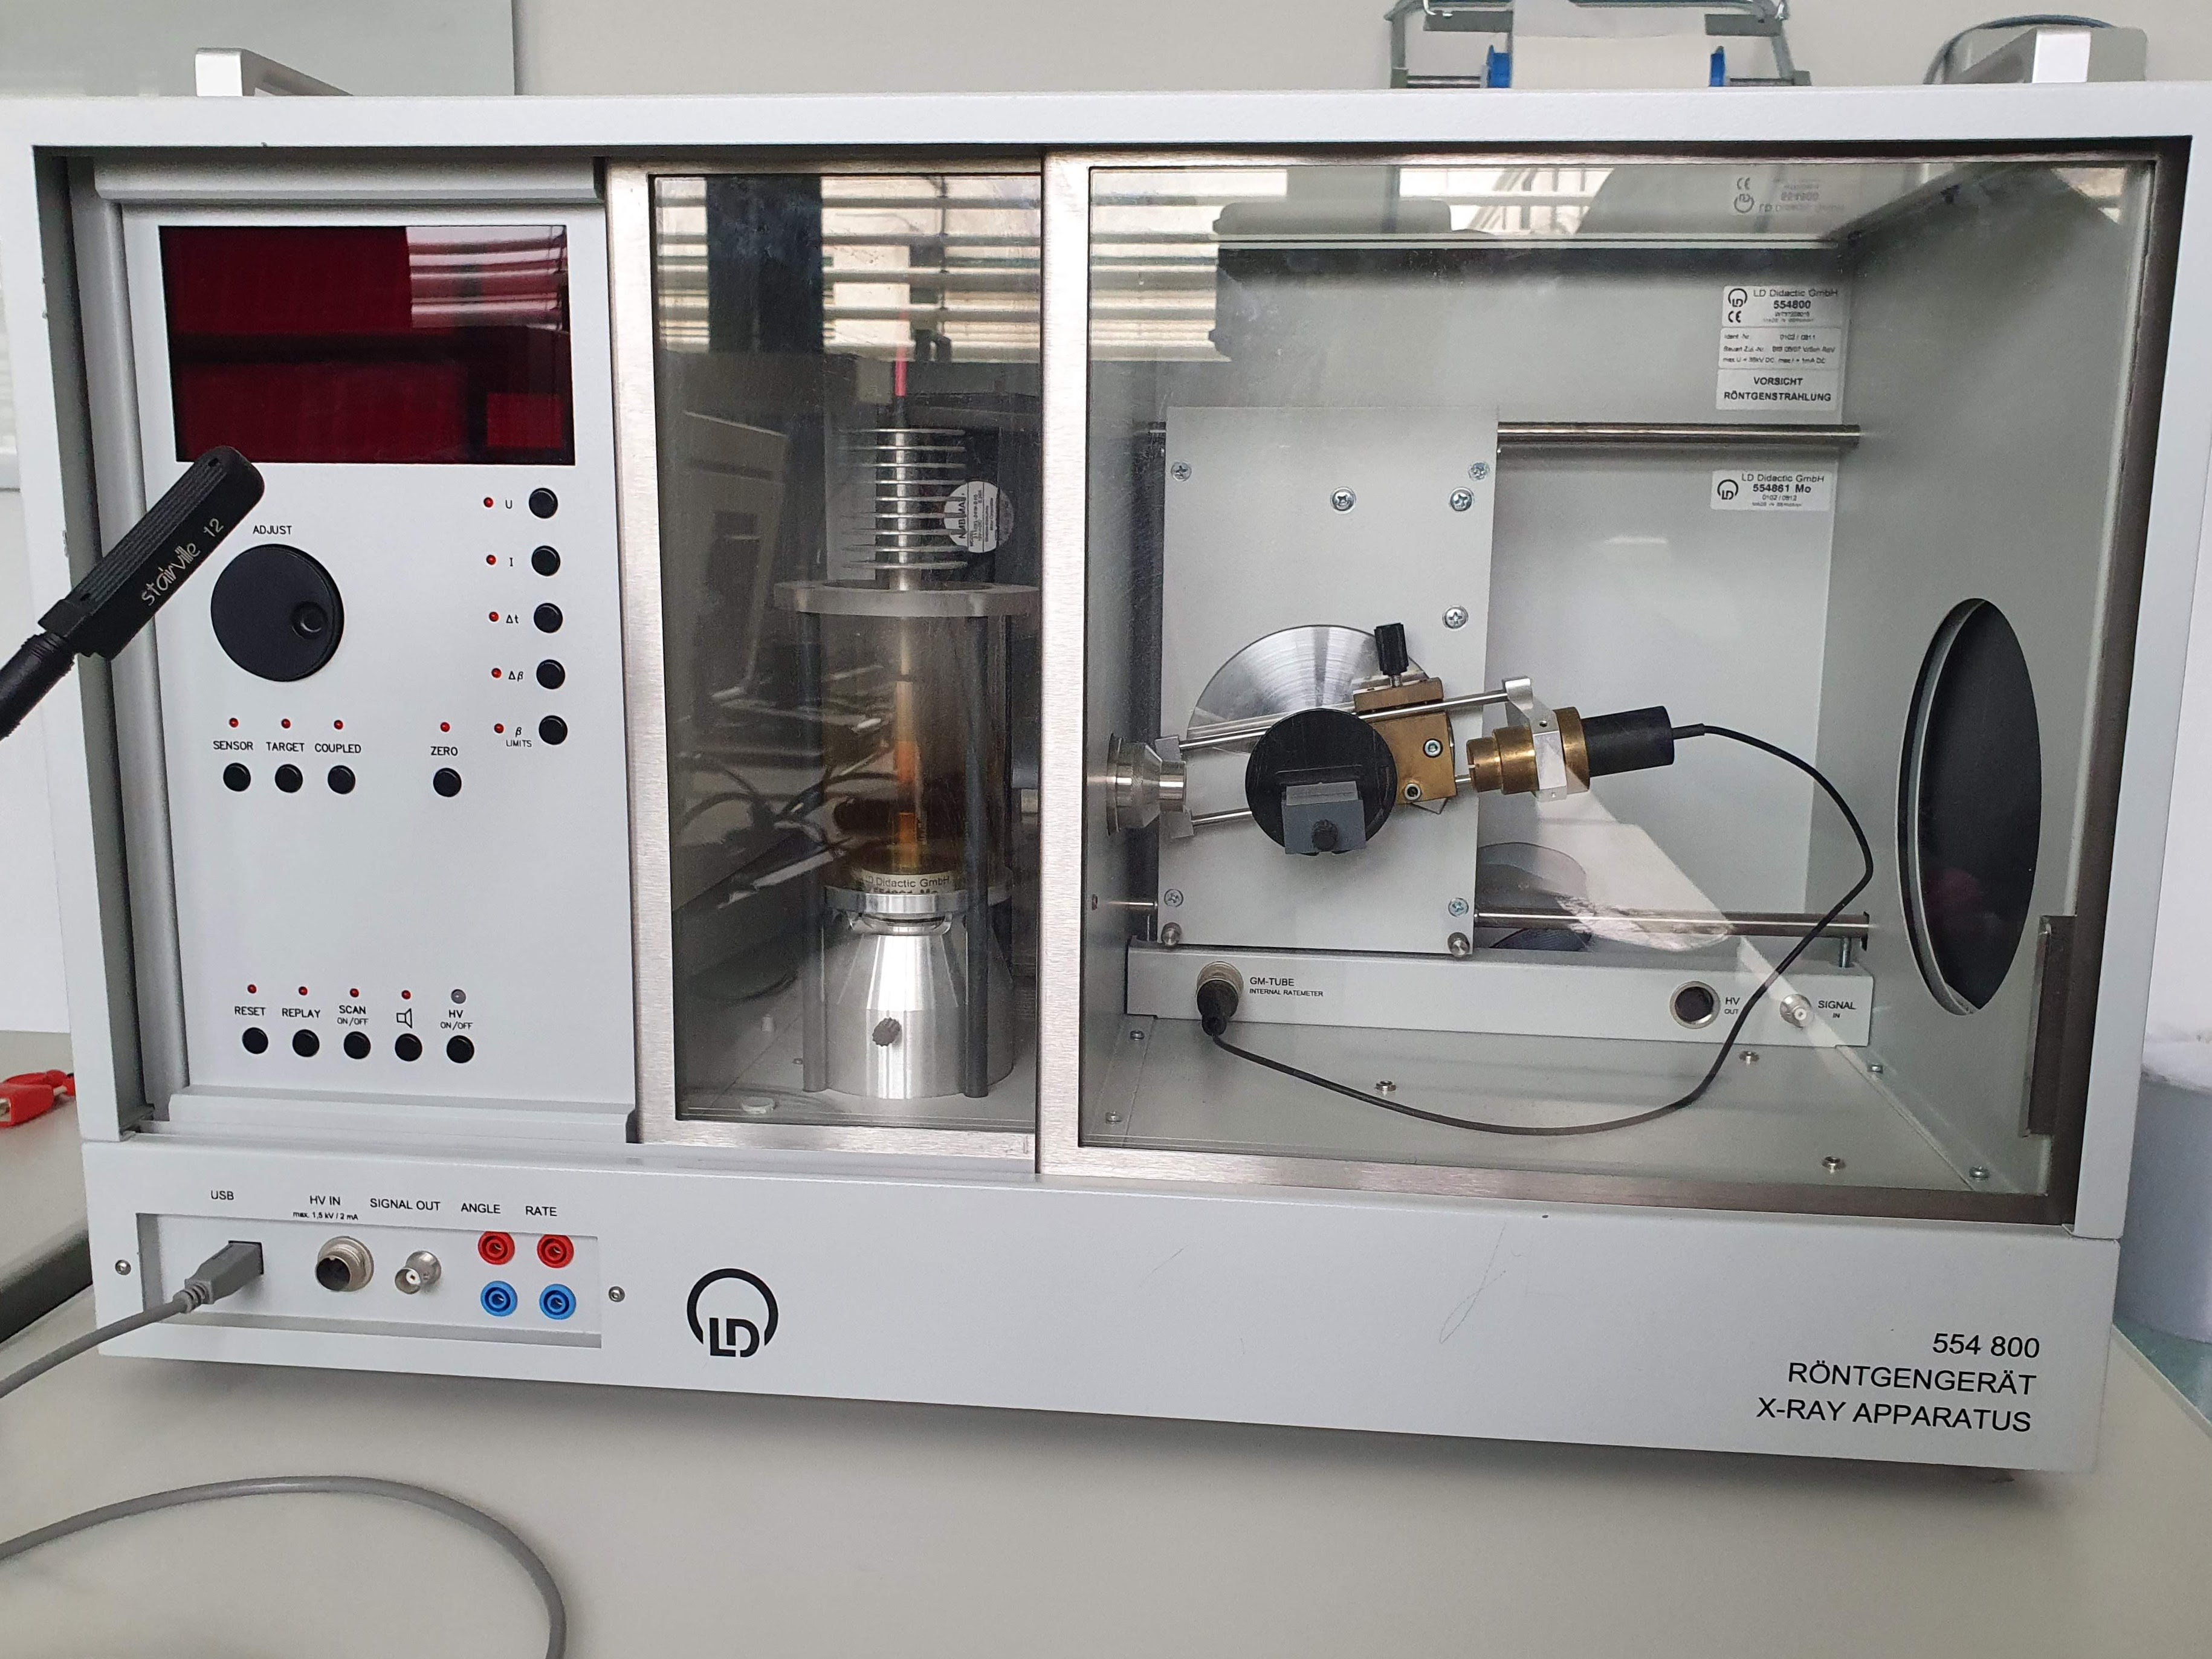
\includegraphics[width=\textwidth]{images/tv1-aufbau.jpg}
			\caption{Röntgengerät}
			% \vspace{0.5\baselineskip}
			\label{fig:tv1-1}
		\end{subfigure}
		\begin{subfigure}{0.48\textwidth}
			\centering
			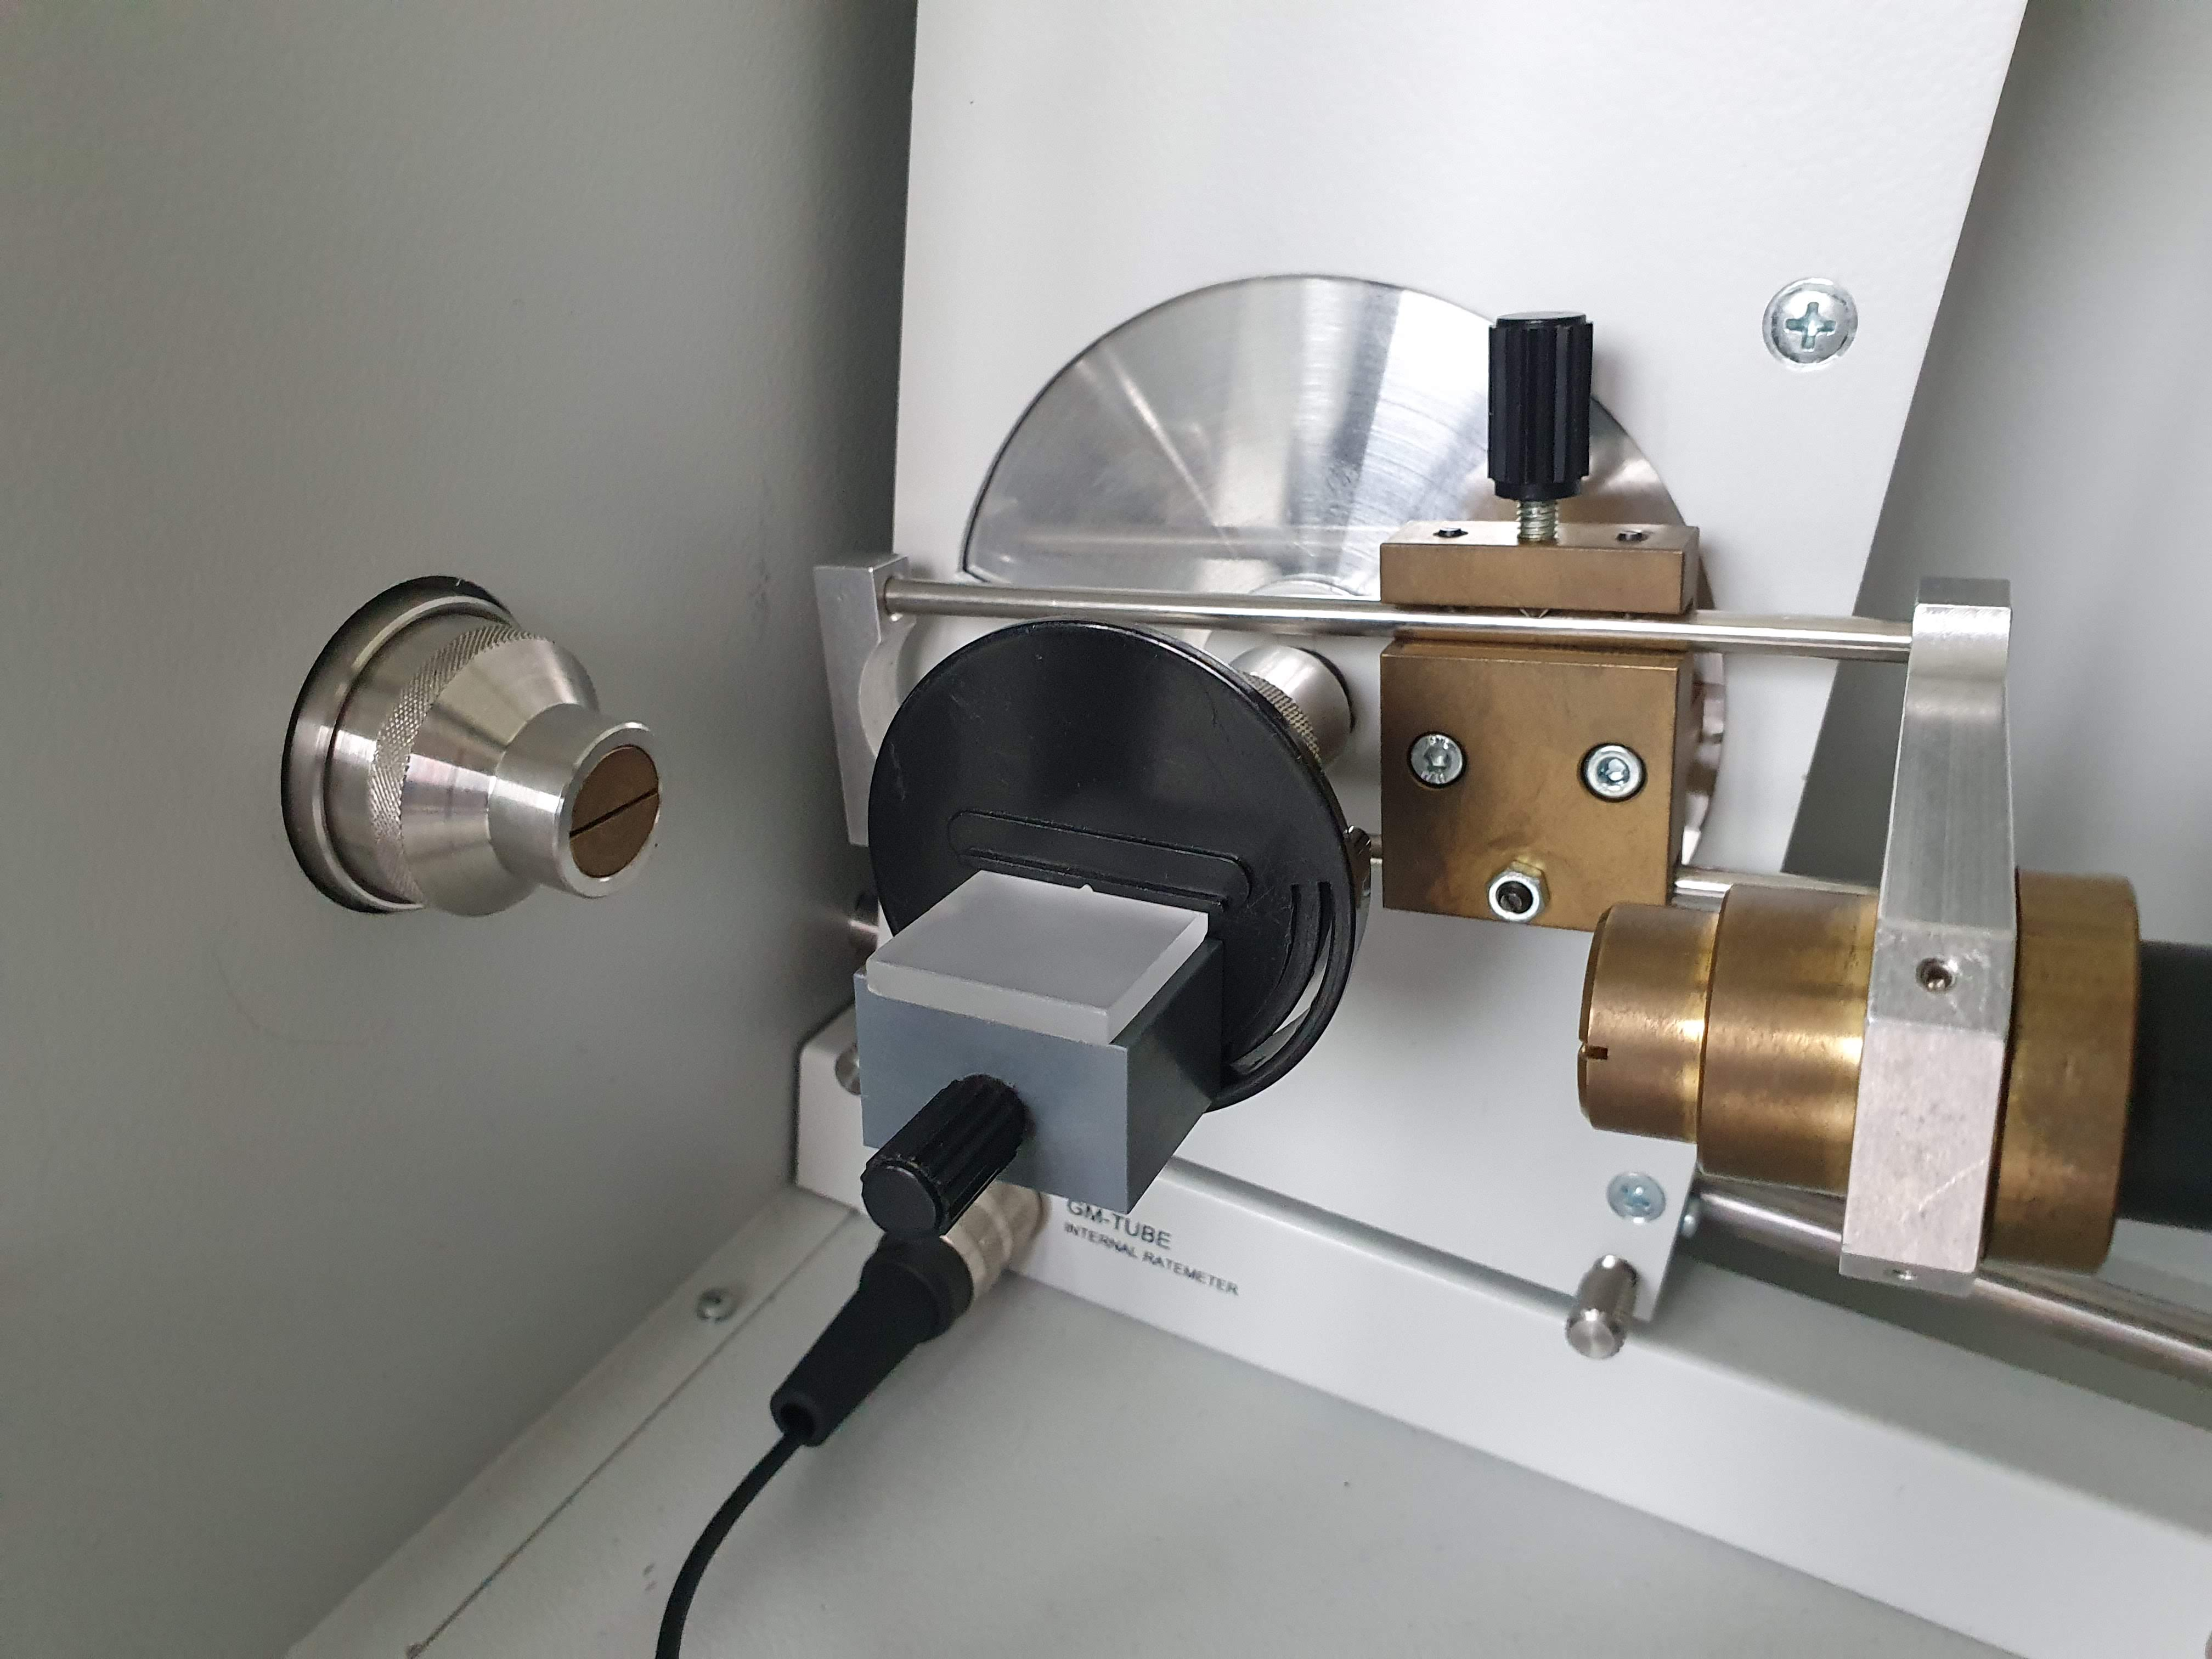
\includegraphics[width=\textwidth]{images/tv1-aufbau2.jpg}
			\caption{Probetisch mit \ce{NaCl}-Einkristall und detektor}
			% \vspace{0.5\baselineskip}
			\label{fig:tv1-2}
		\end{subfigure}
	    \caption{Aufbau von Teilversuch 1}
	\end{figure}
	Wir berechnen zunächst aus unseren $\beta$-Winkeln die entsprechende Wellenlängen. Es gilt:
	\begin{align}
		n\lambda = 2d\sin\beta \notag \\
		\Rightarrow \lambda &= \frac{2d\sin\beta}{n} \\
		\Delta\lambda &= \gausserror{\lambda}{\beta} = \abs{\frac{2d\Delta\beta}{n}\cos{\beta}}
	\end{align}
	wobei alle Winkel in Radian sind. Alle Rechnung erfolgen in LibreOffice Calc.
	\pagebreak
	Um den Mittelwert und Fehler des Mittelwertes zu berechnen, verwenden wir die gerundeten Werten und die Funktion \texttt{AVERAGE} bzw. die Formel:
	\begin{align}
		\Delta \overline{\lambda} = \frac{\addquad{\lambda_1, \lambda_2, \lambda_3}}{3} \label{eqn:tv1-error}
	\end{align}
	wobei der Zähler mithilfe der Funktion \texttt{SUMSQ} in LibreOffice Calc gerechnet ist. 

	Da $n = 3$ noch ziemlich klein ist, ist es nicht sinnvoll die Formel für die Standardabweichung zu verwenden. Die Formel für die Standardabweichung geht von einer gaußschen Verteilung aus, was wir hier nicht gewährleisten können. Wir verwenden somit direkte Fehlerfortpflanzung. 

	Wir erhalten somit:
	\begin{center}
		\vspace{\parskip}
		\begin{tabular}{lrrrr}
			\toprule
			& \multicolumn{2}{c}{$K_\alpha$} & \multicolumn{2}{c}{$K_\beta$} \\
			\cmidrule(lr){2-3} \cmidrule(lr){4-5} % https://tex.stackexchange.com/q/180368
			$n$ & $\beta/\si{\degree}$ & $\lambda/\si{\pico\meter}$ & $\beta/\si{\degree}$ & $\lambda/\si{\pico\meter}$ \\
			\midrule
			$1$ & \num{7.26(12)} & \num{71.3(12)} & \num{6.46(12)} & \num{63.5(12)} \\
			$2$ & \num{14.64(12)} & \num{71.3(6)} & \num{12.96(14)} & \num{63.2(7)} \\
			$3$ & \num{22.24(14)} & \num{71.2(5)} & \num{19.7(8)} & \num{63.38(25)} \\
			\cmidrule(lr){3-3} \cmidrule(lr){5-5}
			& (Mittelwert) & \num{71.3(5)} & (Mittelwert) & \num{63.4(5)} \\
			& ($\lambda_\text{Lit}$) & \num{71.08} & ($\lambda_\text{Lit}$) & \num{63.09} \\
			\bottomrule
		\end{tabular}
		\vspace{\parskip}
	\end{center}
	Die experimenlle Werten stimmen mit der Literaturwerten überein.


\newpage
\section{Teilversuch 2: Kalibrierung des Linsensystems}
	\begin{figure}[!ht]
	    \centering
	    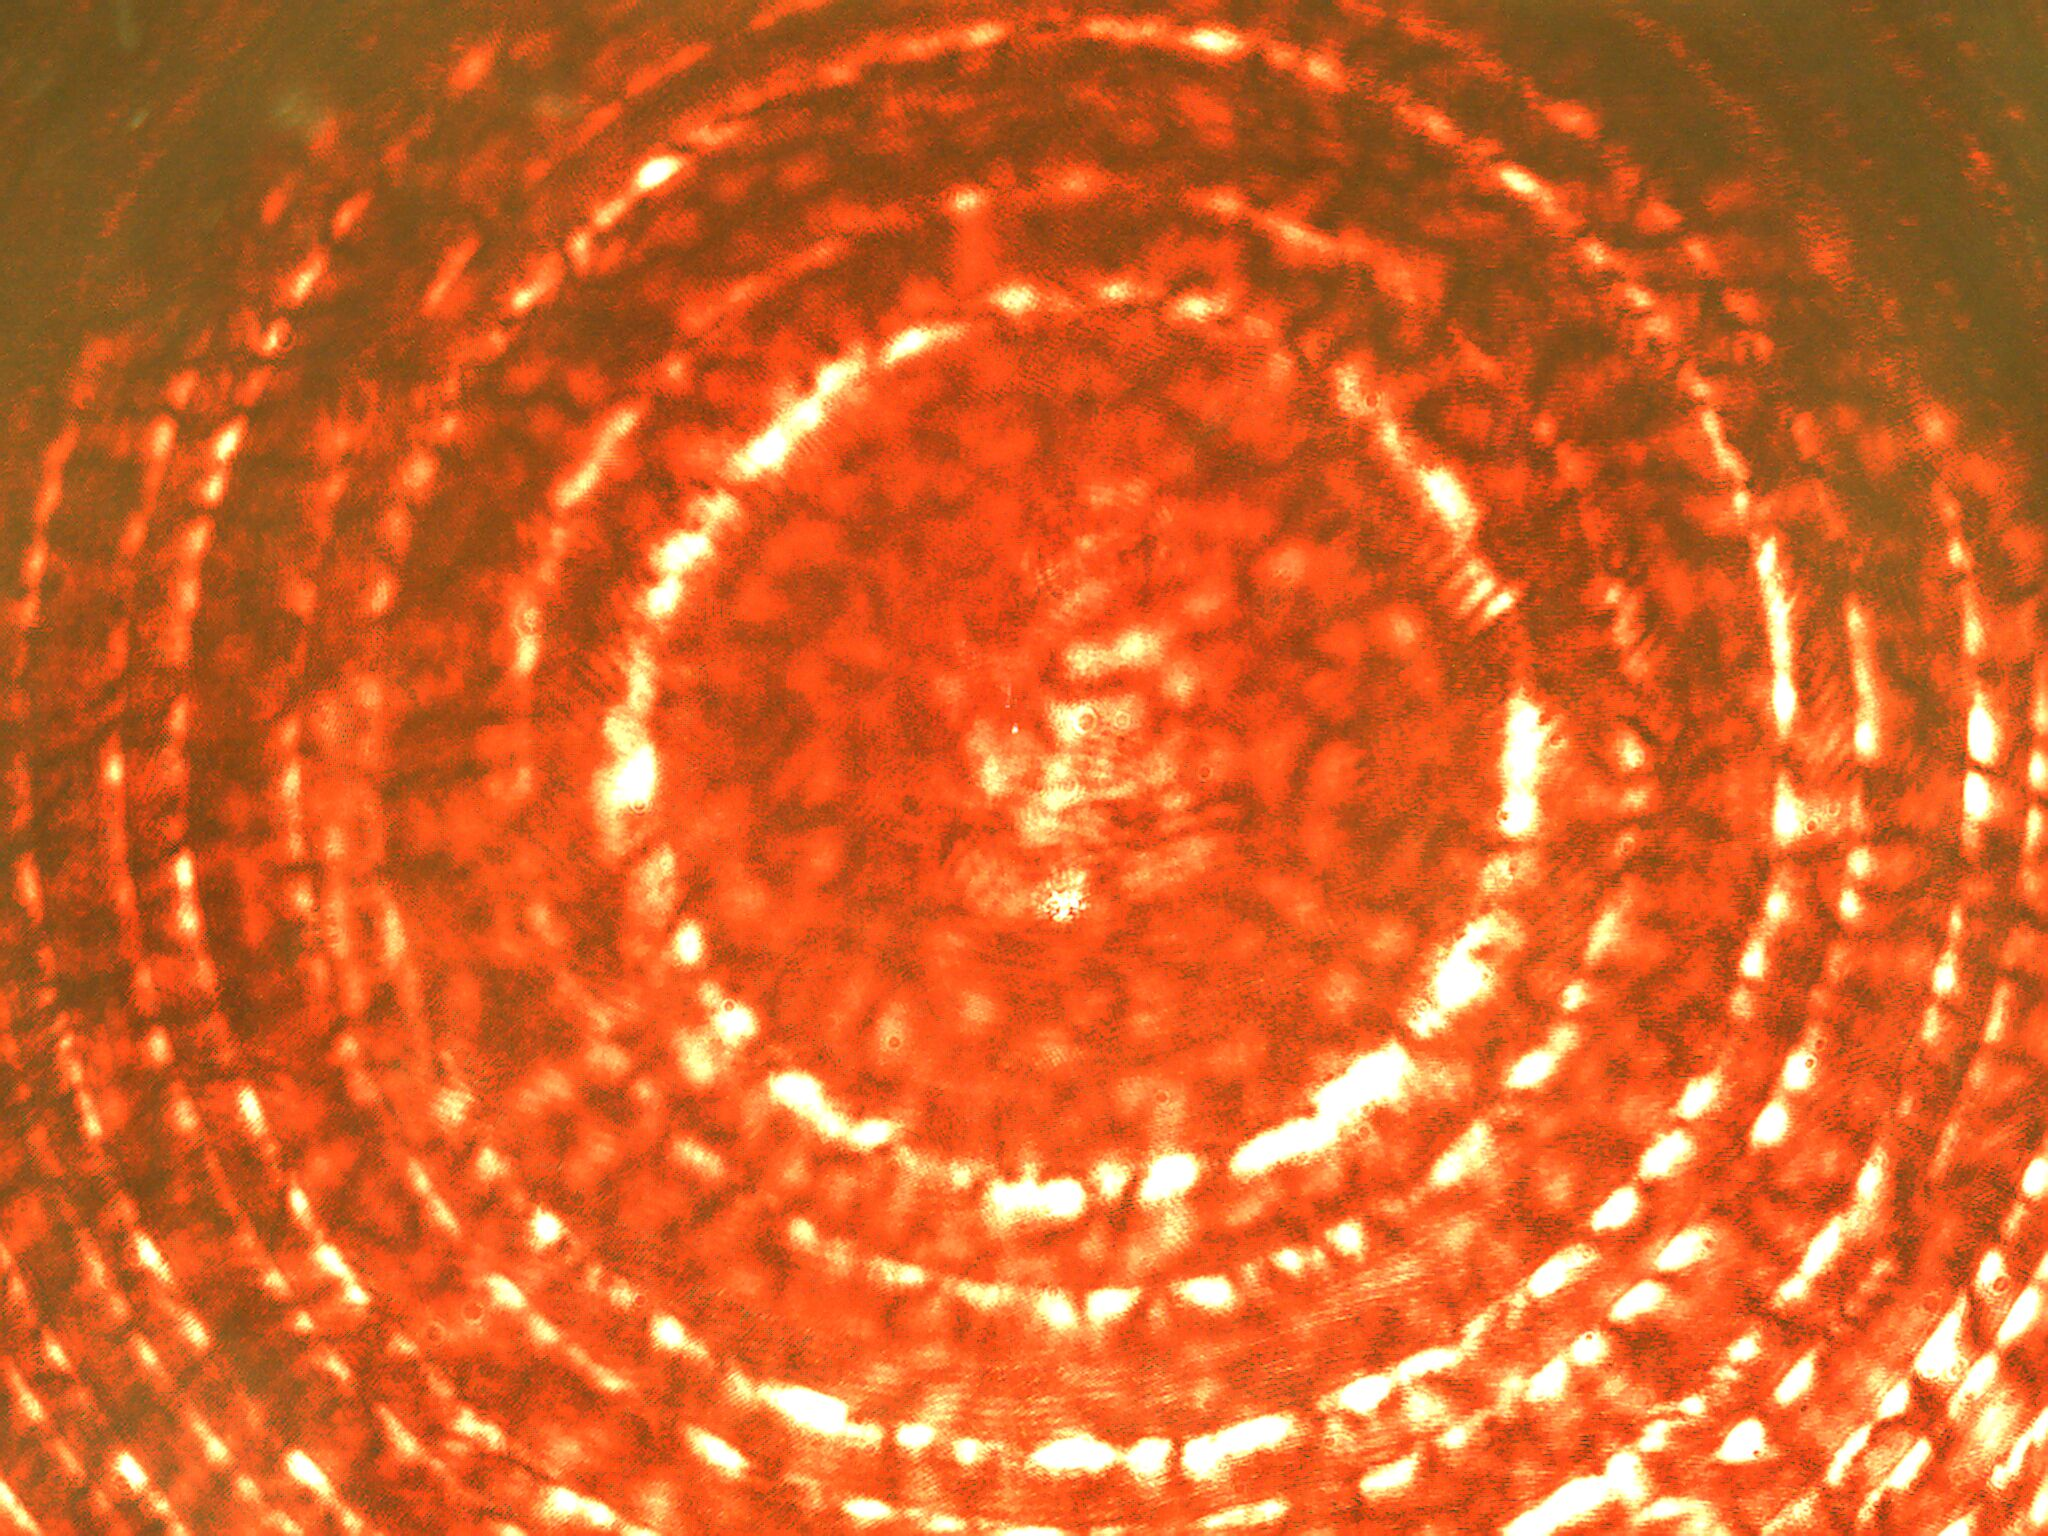
\includegraphics[width=0.7\textwidth]{images/Capture_807.bmp.jpg}
	    \caption{Interferenzringe mit Laserpointer}
	    \label{fig:laser-interference}
	\end{figure}
\newpage
\section{Teilversuch 3: Duane-Huntsches Verschiebungsgesetz}
	Auf der Kurveanpassungen erhalten wir die Messreihe:
	\begin{center}
		\vspace{\parskip}
		\begin{tabular}{l*{8}{r}}
		\toprule
			$U/\si{\kilo\volt}$ & \num{35} & \num{34} & \num{32} & \num{30} & \num{28} & \num{26} & \num{24} & \num{22} \\
		\midrule
			$\lambda_\text{min}/\si{\pico\meter}$ & \num{33.8} & \num{34.8} & \num{37.0} & \num{39.8} & \num{42.7} & \num{46.1} & \num{49.4} & \num{53.8} \\
		\bottomrule			
		\end{tabular}
		\vspace{\parskip}
	\end{center}
	Es ist kein Fehler im Programm angegeben. Es erfolgt also keine Fehlerrechnung.

	Wir haben nach der Kurveanpassung im Programm die folgende Ergebnis bekommen:
	\begin{center}
		\begin{tabular}{llr}
			\toprule
			\multicolumn{2}{l}{Variable} & Wert \\
			\midrule
			$A$	& Steigung& \SI{1190}{\pico\meter\kilo\volt} \\
			$h$	& Plancksches Wirkungsquantum & \SI{6.36e-34}{\joule\second} \\
			\bottomrule 
		\end{tabular}
	\end{center}
	Es gilt:
	\begin{align}
		\lambda_\text{min} = \frac{hc}{e}\left(\frac{1}{U}\right) &&\implies&& A = \frac{hc}{e}
	\end{align}
	Somit können wir das Plancksche Wirkungsquantum aus der Steigung ermitteln, was das Programm uns schon gemacht hat. Das Ergebnis von $h_\text{exp} = \SI{6.36e-34}{\joule\second}$ ist sehr nah an $h_\text{Lit} = \SI{6.626e-34}{\joule\second}$. Da es keine Unsicherheit vorhanden ist, können wir keine Aussage darüber schließen, ob die zwei Werte miteinander verträglich sind. Da die Werte aber sehr nah an andere sind, stimmen das Duane-Huntsches Verschiebungsgesetz. 

	Eine mögliche Fehlerquelle ist die ungenaue Bestimmung des linearen Anteils der Kurve. Die Grenzwellenlänge $\lambda_\text{min}$ ist aber stark von der Kurveanpassung abhängig. Somit kann diese ungenaue Bestimmung zu Fehler in der Grenzwellenlänge führen.



\resnum
% \newpage
\appendix
%  Bibliography
    % \renewcommand*{\bibfont}{\raggedright}
    % \urlstyle{sf}
    % \hypersetup{urlcolor=gray}
    % \printbibliography
% / Bibliography

\section{\gnuplot{} Quellcode zur Auswertung von Teilversuch 1b}
    Wir verwenden hier immer die Datei \texttt{tv1.dat}:
        \begin{minted}[linenos,breaklines,autogobble,frame=leftline,framesep=10pt]{text}
# Peak  f/Hz    A/au    width/Hz phase/deg
1   5719,715    59,0441 17,634   -46,7
2   6853,203    41,929  18,732   -1,7
3   7989,781    31,0203 19,371   29,9
4   9124,208    22,639  20,437   57,9
5   10259,772   14,1618 22,807   63,8
6   11393,832   13,2206 23,386   90,7
7   12524,178   9,5492  27,648   98,3
8   13641,917   7,4138  33,978   133,8
        \end{minted}
    \subsection{Regelmäßiger Abstand}
    \label{appdx:tv1-1}
    {  
        % % Surpress "errors" in minted
        % https://tex.stackexchange.com/a/289068
        \renewcommand{\fcolorbox}[4][]{#4}
        \inputminted[linenos,breaklines,autogobble,frame=leftline,framesep=10pt]{gnuplot}{plots/tv1-1.gp}
    }
    Rohausgabe:
    \inputminted[linenos,breaklines,autogobble,frame=leftline,framesep=10pt]{text}{plots/tv1-1.gp.out}
    \subsection{Lebensdauer}
    \label{appdx:tv1-2}
    {  
        % % Surpress "errors" in minted
        % https://tex.stackexchange.com/a/289068
        \renewcommand{\fcolorbox}[4][]{#4}
        \inputminted[linenos,breaklines,autogobble,frame=leftline,framesep=10pt]{gnuplot}{plots/tv1-2.gp}
    }
    Rohausgabe:
    \inputminted[linenos,breaklines,autogobble,frame=leftline,framesep=10pt]{text}{plots/tv1-2.gp.out}

\section{\gnuplot{} Quellcode zur Auswertung von Teilversuch 2a}
    \label{appdx:tv2a}
    {  
        % % Surpress "errors" in minted
        % https://tex.stackexchange.com/a/289068
        \renewcommand{\fcolorbox}[4][]{#4}
        \inputminted[linenos,breaklines,autogobble,frame=leftline,framesep=10pt]{gnuplot}{plots/tv2a.gp}
    }
    mit \texttt{tv2a.dat}:
    \begin{minted}[linenos,breaklines,autogobble,frame=leftline,framesep=10pt]{text}
# alpha Theta           A3,663  A4,950  A6,190
180 180                 0,373   0,539   -0,303
170 172,933425610738    0,356   0,528   -0,279
160 165,893955739434    0,331   0,474   -0,211
150 158,909418821001    0,295   0,375   -0,103
140 152,009109282217    0,243   0,244   0,011
130 145,224563330281    0,189   0,091   0,103
120 138,590377890729    0,138   -0,052  0,169
110 132,145070558482    0,031   -0,151  0,187
100 125,93195832035     0,031   -0,225  0,169
90  120                 0,042   -0,259  0,117
80  114,404497337886    0,078   -0,269  0,046
70  109,207479725344    -0,128  -0,236  0,029
60  104,47751218593     -0,105  -0,185  -0,071
50  100,288585136763    -0,182  -0,119  -0,091
40  96,7177134641804    -0,167  -0,055  -0,085
30  93,8409657162581    -0,189  -0,099  -0,065
20  91,7279410723505    -0,202  -0,069  -0,040
10  90,4352300024699    -0,205  -0,099  -0,030
0   90                  -0,210  -0,112  0,032
        \end{minted}
    Rohausgabe:
    \inputminted[linenos,breaklines,autogobble,frame=leftline,framesep=10pt]{text}{plots/tv2a.gp.out}
\end{document}
